

\section{A new perspective on SUPG}
Partial differential equations exhibiting multi-scale behavior are notoriously difficult to approximate numerically. In the functional analysis setting the issue is often characterized by a loss of discrete stability (coercivity) of the bilinear form in question. We develop a continuous Petrov Galerkin method that provides a stable and accurate solution in a norm of choice.  This is achieved by computing compactly supported continuous test-functions that are the solution to a small local adjoint problem in an enriched space subject to a projector of choice. Computation of such functions is still relatively expensive. We create a database of optimal test functions for a range of flows and train a simplified model using  machine learning techniques in order to approximate their action.

\subsection{Optimal test functions}
Let $\Omega \subset \mathbb{R}^{n_{sd}}$ be an open set and $V$ an infinite dimensional Hilbert space with, for simplicity, homogeneous Dirichlet boundary conditions on $\Omega$. Suppose we wish to solve the following boundary value problem:  find $ u \in V$ such that,
\begin{align}
	a(u,v) + b(u,v) &= l(v) \quad \forall v \in V
	\label{eq:problem}
\end{align}
where $a(\cdot, \cdot)$ is a positive definite symmetric and $b(u,v)$ a is skew symmetric bilinear form and $l(\cdot )$ is a linear form on $V$.

Consider the direct sum decomposition of $V$:
\begin{align}
	V = \overline{V} \oplus V'
	\label{eq:decomp}
\end{align}
where $\overline{V}$ is thought of as the coarse scale subspace of $V$ and $V'$ as the corresponding fine-scale subspace. This scale separation is performed by means of a linear projector.
\begin{definition} Let  $\mathcal{P} \; : \; V \mapsto \overline{V}$ be a linear projector defined by means of the following linear boundary value problem: given $u \in V$, find $\bar{u} = \mathcal{P}(u)$ such that.
\begin{align}
	a(u- \bar{u}, \bar{v}) = 0 \quad \forall \bar{v} \in \overline{V}
	\label{eq:proj}
\end{align}
\end{definition}

We wish to discretize (\ref{eq:problem}) using a Petrov-Galerkin method that is discretely stable (coercive) and is close to the best approximation of the analytical solution $u \in V$ in the norm subject to the projector $\mathcal{P}$: find $\bar{u} \in \overline{V}$ such that,
\begin{align}
	a(\bar{u},\bar{w}) + b(\bar{u},\bar{w}) &= l(\bar{w}) \quad \forall \bar{w} \in \overline{W}
	\label{eq:problem2}
\end{align}
where $\overline{W} \subset V$ is another finite dimensional space that is in general not the same as $\overline{V}$ and is yet to be determined. 

\begin{definition} Let $ \phi_i(x) \in \overline{V}, \; i=1,2,...,n$ be a set of linearly independent shape functions. We define,
\begin{align}
	 \overline{V} := \mathrm{span} \left\{ \phi_i(x), \; i=1,2,...,n   \right\} 
\end{align}
\end{definition}

\begin{theorem} Let  the solution to the Petrov Galerkin method in (\ref{eq:problem2}) be equal to $\bar{u} = \mathcal{P}(u)$. Then, the space of test functions is given as follows,
\begin{align}
	& \overline{W} := \mathrm{span} \left\{ \phi_i(x) +  \psi_i(x), \; i=1,2,...,n   \right\} &
\end{align}
where $\phi_i(x) +  \psi_i(x), \; i=1,2,...,n$ is linearly independent and the latter follows from the following adjoint problem: find $\psi_i \in V'$, $i=1,2,...,n$, such that,
\begin{align}
 a(u', \psi_i) + b(u', \psi_i) = - b(u', \phi_i)  \quad \forall u' \in V'.
 \label{eq:problem3}
\end{align}
\end{theorem}
\begin{proof} Using the property (\ref{eq:proj}) of the projector  and Galerkin orthogonality, we obtain,
\begin{align}
	a(u', \phi_i)  = a(u', \phi_i + \psi_i) + b(u', \phi_i + \psi_i) &= 0 \quad \forall u' \in V'.
\end{align}
for $i=1,2,...,n$. This leads directly to the relation in (\ref{eq:problem3}). Since $\phi_i \in \overline{V}$, $i=1,2,...$ is a linearly independent set of basis functions and $\psi_i \in V'$ is not in $V$, we have that $\phi_i + \psi_i, \; i=1,2,...,n$ is linearly independent as well. Hence, its use in the Petrov Galerkin scheme yields the solution $\bar{u} = \mathcal{P}(u)$.
\end{proof}

\begin{remark} Since the discrete solution $\bar{u} \in \overline{V}$ coming from the Petrov Galerkin method in (\ref{eq:problem2}) is equal to $\bar{u} = \mathcal{P}(u)$, we have that the set of discretized equations is discretely stable (coercive) and has a best approximation property in the norm defined by $\mathcal{P}$.
\end{remark}

Up to this point no approximations have been made. For practical reasons we would like that the test functions $ \left\{ \phi_i(x) +  \psi_i(x), \; i=1,2,...,n   \right\} $ have local support. A natural choice would be to choose,
\begin{align}
	\psi_i(x) = 0 \quad \text{if } x \notin \mathrm{supp} \; \phi_i, \quad i = 1,2,...,n.
	\label{eq:compactsupp}
\end{align}
This is what we shall assume in the following.
\begin{remark} At first sight the problem in (\ref{eq:problem3}) is equally difficult to solve as the original problem. Note however that with the assumption of compact support (\ref{eq:compactsupp}) we have that,
	\begin{enumerate} 
		\item The problem in (\ref{eq:problem3}) is local to the domain $\Omega_i:=\mathrm{supp} \left(  \phi_i \right) \subset \Omega$ for $i=1,2,...,n$.
		\item Homogeneous boundary conditions.
		\item The problem in (\ref{eq:problem3}) is linear even if the original problem in (\ref{eq:problem}) is non-linear. 
	\end{enumerate}
\end{remark}

\begin{remark} Optimal test functions $\phi_i+\psi_i, \; i=1,2,...,n$ can be numerically computed on a sub scale discretization local to the domain $\Omega_i:=\mathrm{supp} \left(  \phi_i \right) \subset \Omega$. 
\end{remark}

\begin{remark} The proposed Petrov Galerkin scheme reduces to standard Galerkin in the case of a pure diffusion problem. 
\end{remark}

\begin{remark} $b(\phi_i, \psi_j)$  is positive definite and symmetric. I still need to prove this. Hence, this is the term that provides the stability.
\end{remark}

Below follow some initial results using linear and quadratic finite elements. Figures \ref{fig:optimaltestfunc1} and \ref{fig:optimaltestfunc2} illustrate the computation of the optimal test functions for a two element partition. Figure \ref{fig:optimaltestfunc3} computes the numerical solution using this same basis for an advection diffusion problem with $Pe = 10$. Finally Figures \ref{fig:optimaltestfunc4} and \ref{fig:optimaltestfunc5} compute the numerical solution on a ten element partition to an advection diffusion problem with $Pe = 500$ and homogeneous and non-homogeneous right-hand-side, respectively. 
\begin{figure}
	\centering
	\subfigure[$p = 1$]{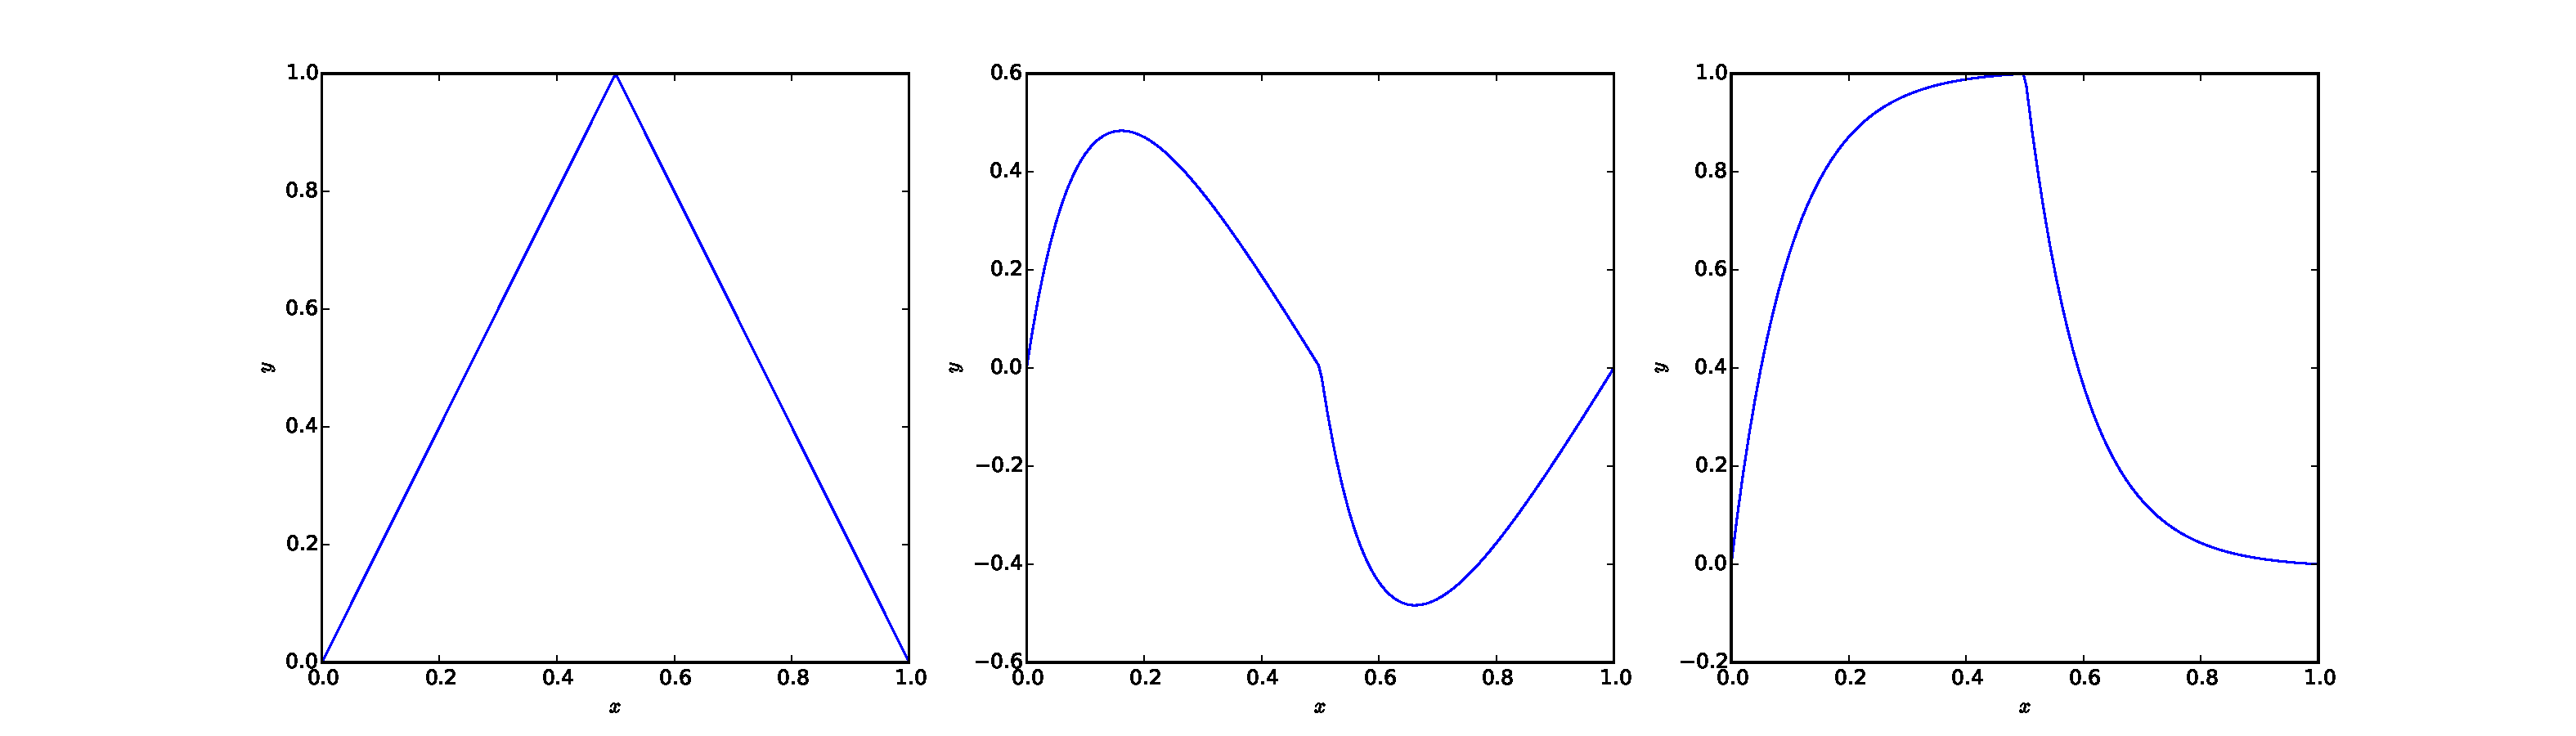
\includegraphics[trim = 0cm  0cm 0cm 0cm,clip,width=1\textwidth]{figures/optimaltestfunction_degree_1_Peclet_10}} \\
	\subfigure[$p = 2$]{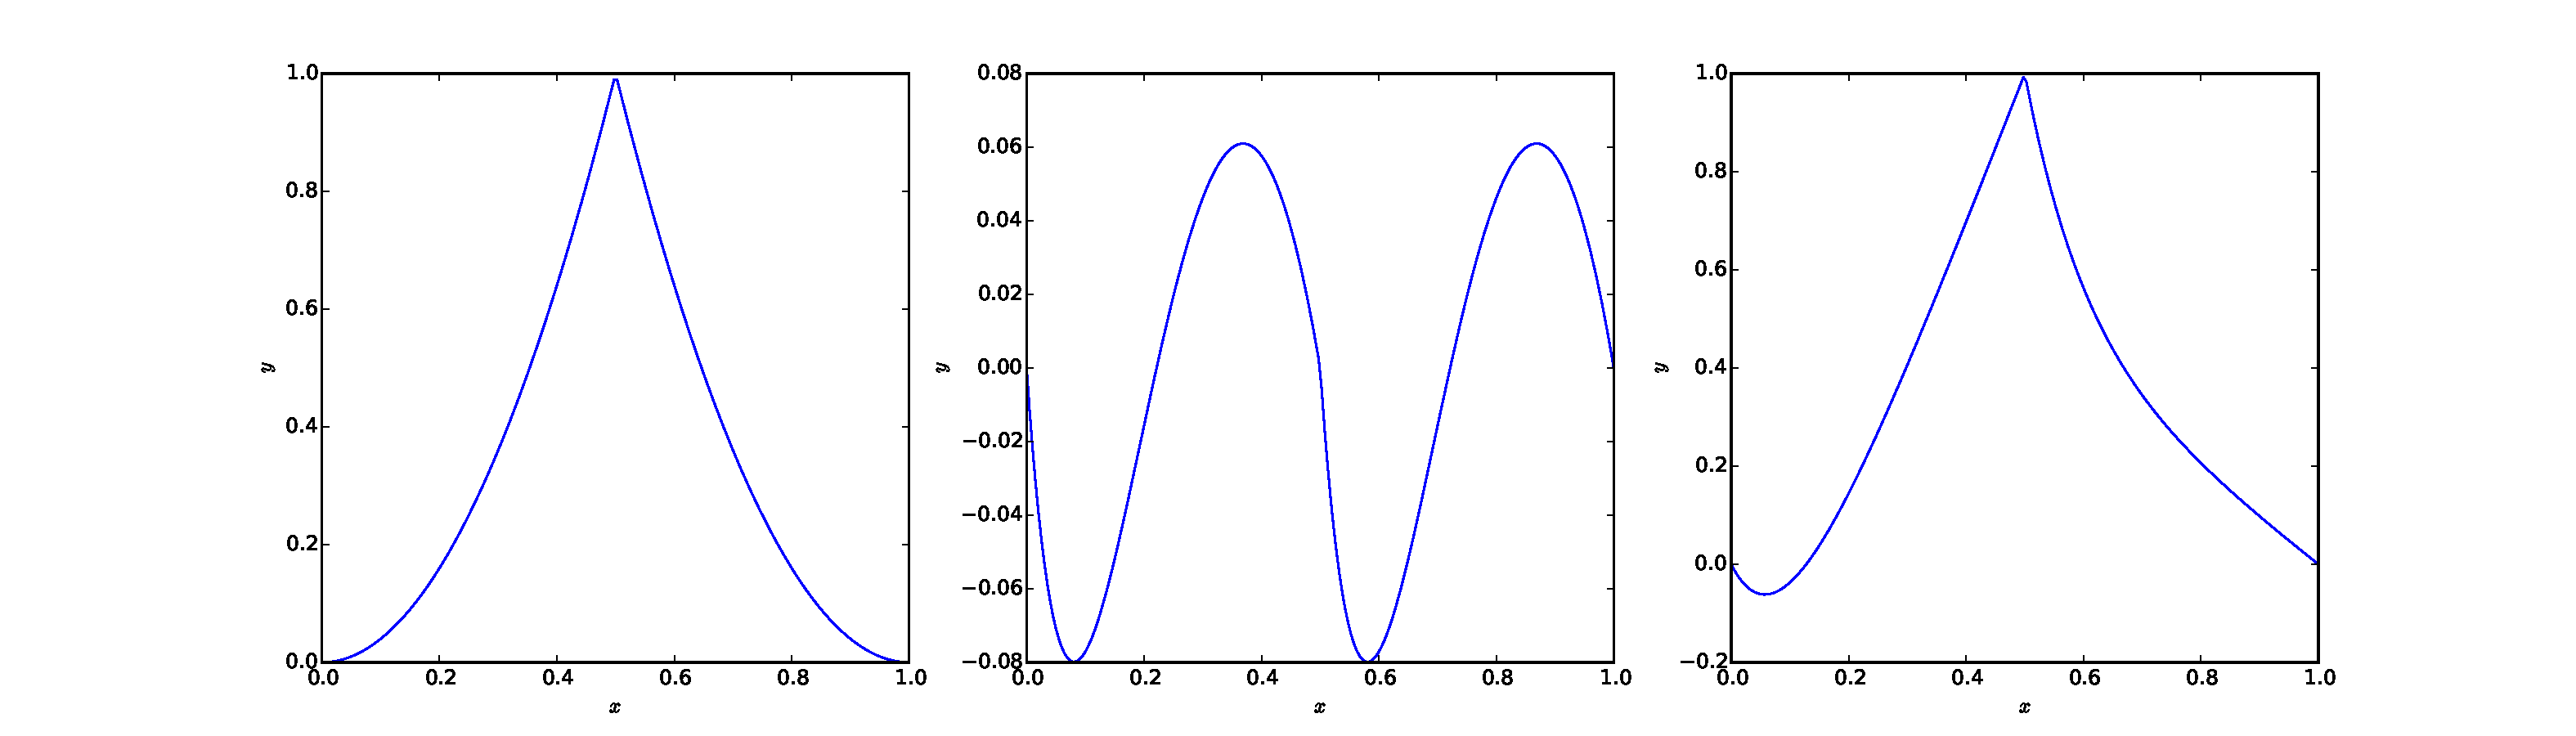
\includegraphics[trim = 0cm  0cm 0cm 0cm,clip,width=1\textwidth]{figures/optimaltestfunction_degree_2_Peclet_10}} 
	\caption{Calculation of optimal test-functions in the $H^1_0$ semi-norm for linear and quadratic finite elements at $Pe=10$. (Left) Coarse scale function $\bar{\phi}_i$. (Middle)  fine scale part $\psi_i'$. (Right) optimal test-function as the sum of the coarse scale function and a fine scale part $\bar{\phi}_i + \psi_i'$.}
	\label{fig:optimaltestfunc1}
\end{figure}

\begin{figure}
	\centering
	\subfigure[$p = 1$]{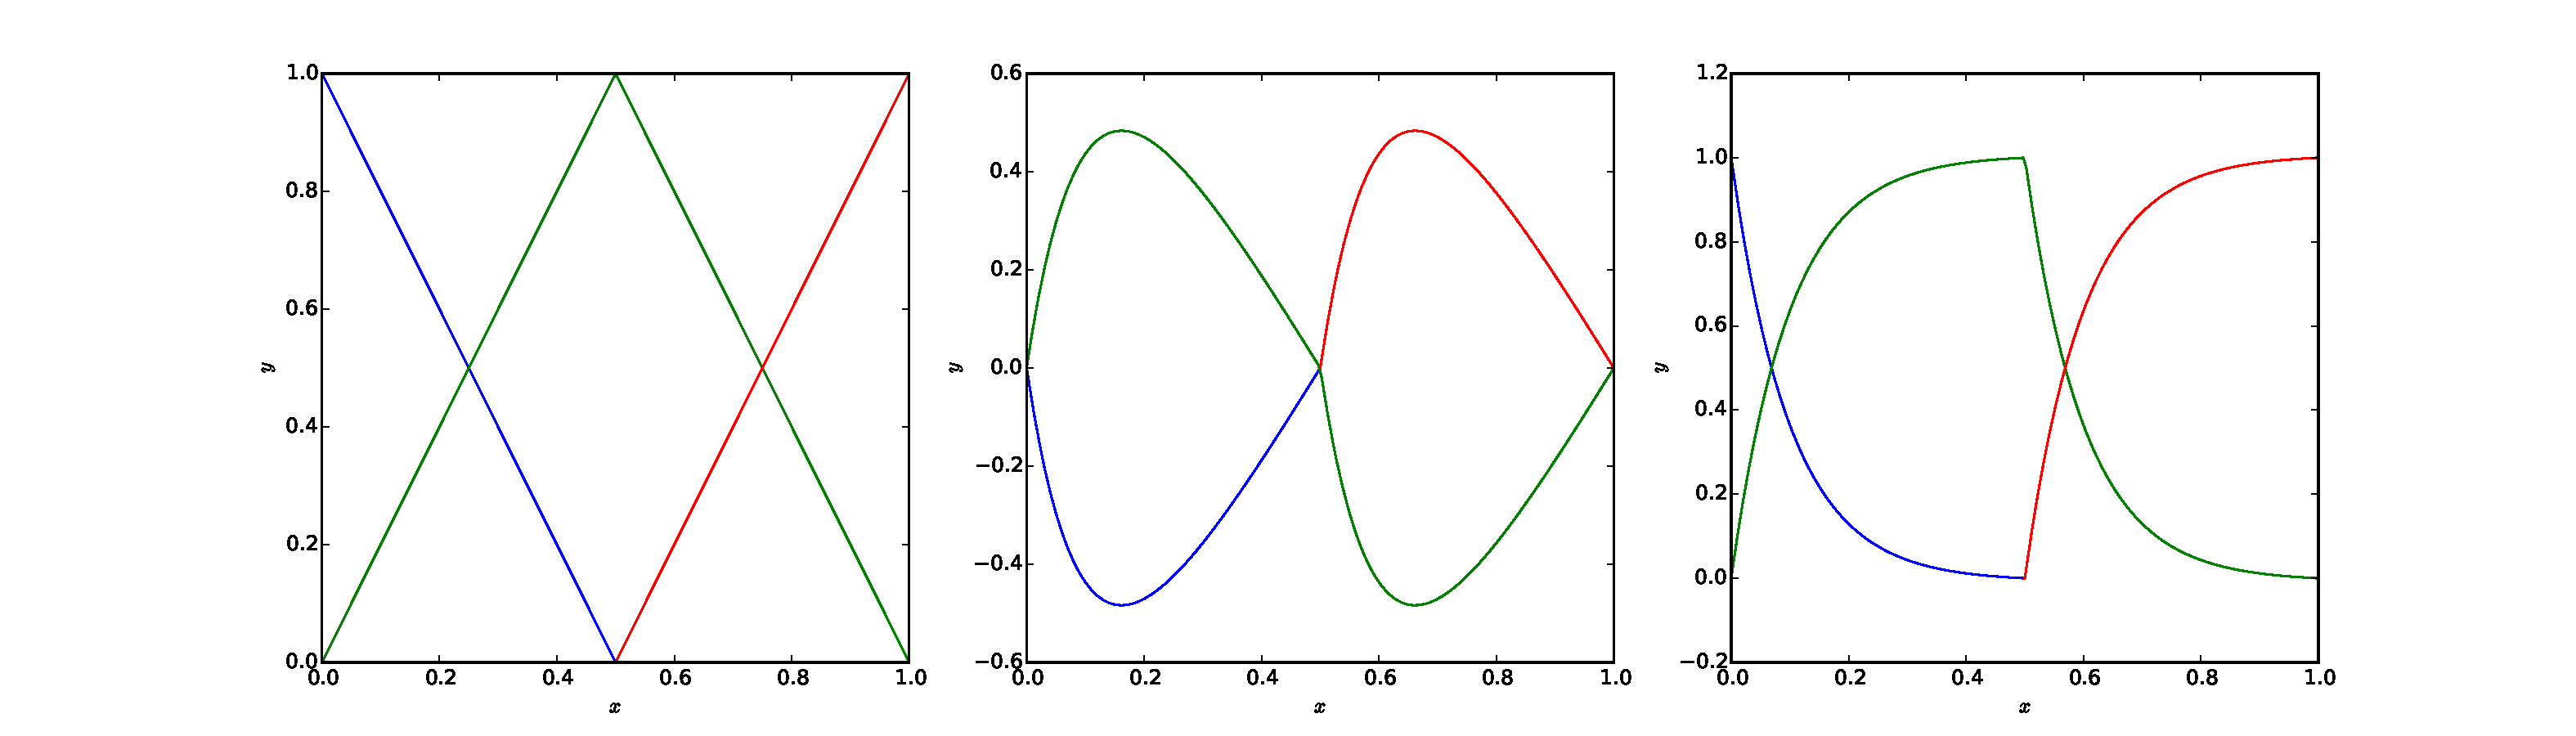
\includegraphics[trim = 0cm  0cm 0cm 0cm,clip,width=1\textwidth]{figures/optimaltestbasis_degree_1_Peclet_10}} \\
	\subfigure[$p = 2$]{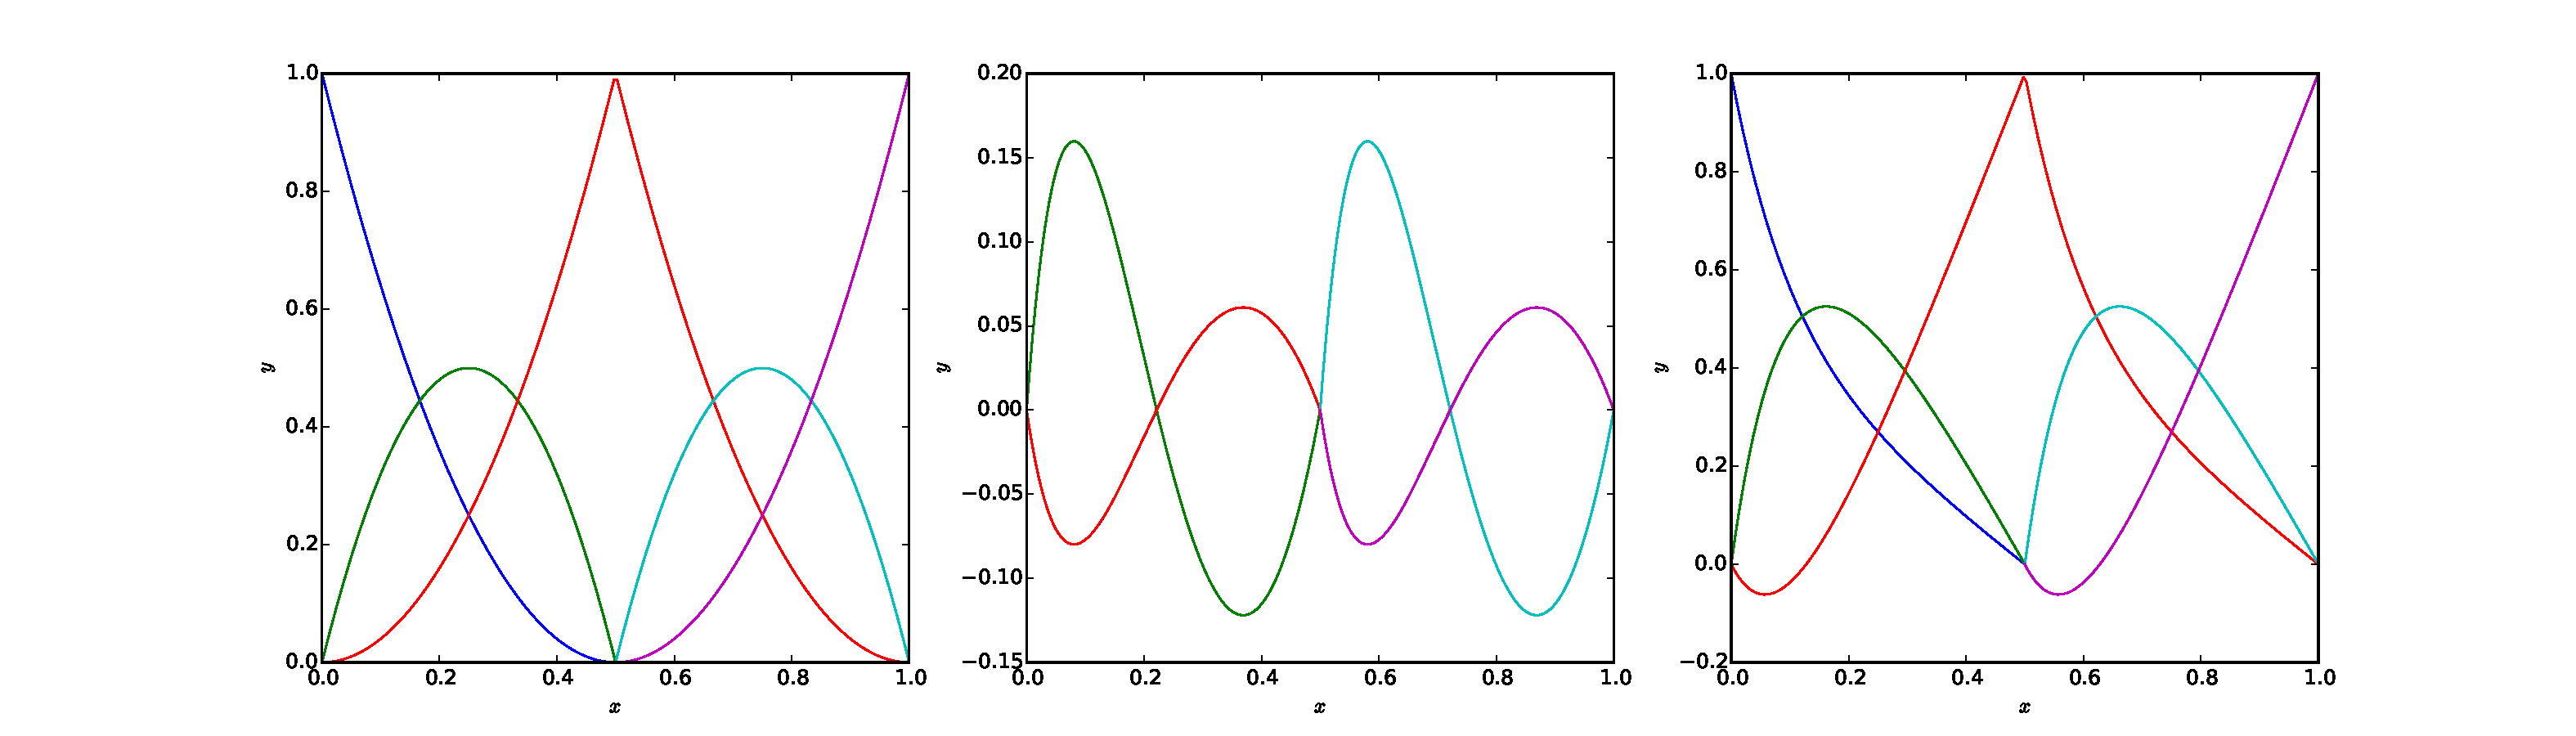
\includegraphics[trim = 0cm  0cm 0cm 0cm,clip,width=1\textwidth]{figures/optimaltestbasis_degree_2_Peclet_10}} 
	\caption{Optimal basis in the $H^1_0$ semi-norm for the test-space for linear and quadratic finite elements at $Pe=10$. (Left) Basis for the coarse scales. (Middle)  part due to the fine scale behaviour. (Right) optimal basis as the sum of the coarse scale function and a fine scale part.}
	\label{fig:optimaltestfunc2}
\end{figure}

\begin{figure}
	\centering
	\subfigure[$p = 1$]{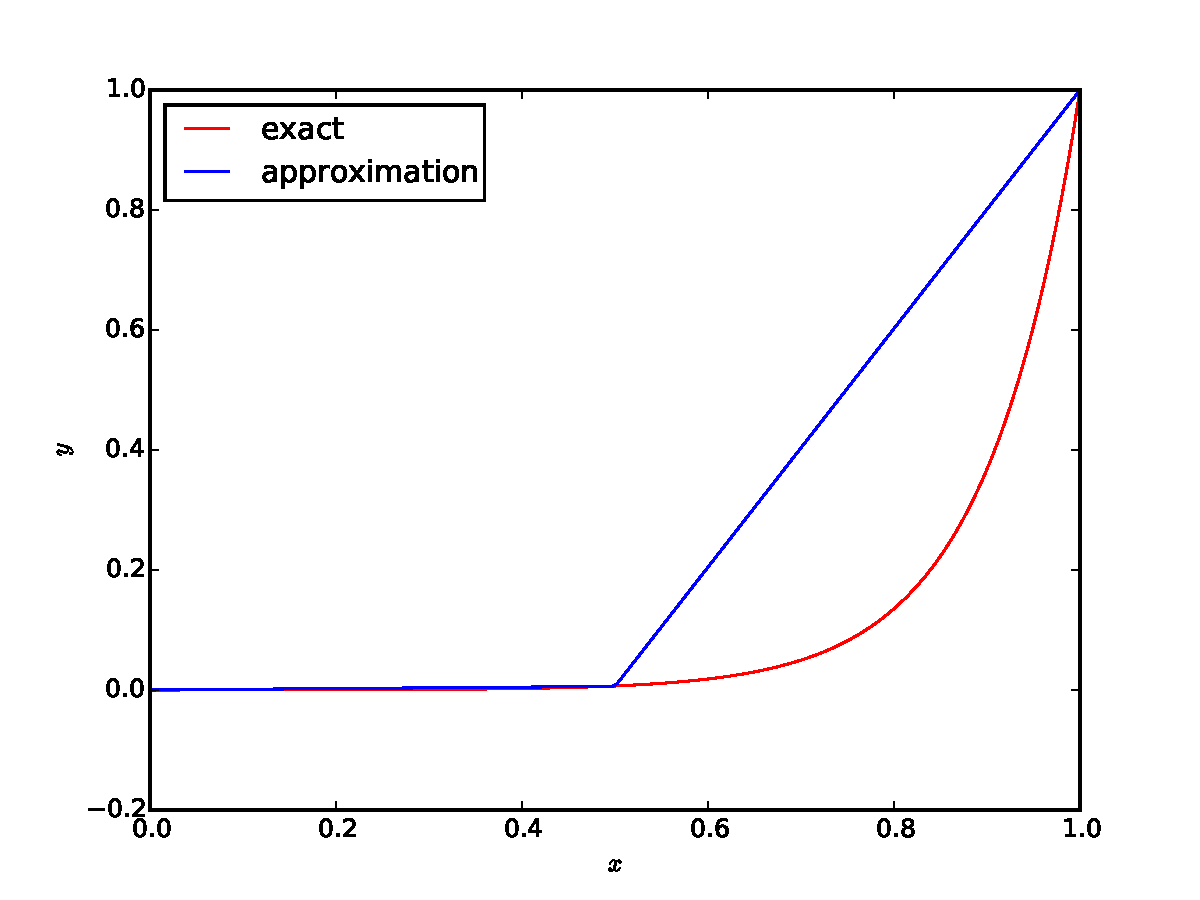
\includegraphics[trim = 0cm  0cm 0cm 0cm,clip,width=0.49\textwidth]{figures/optimalsolution_degree_1_Peclet_10}}
	\subfigure[$p = 2$]{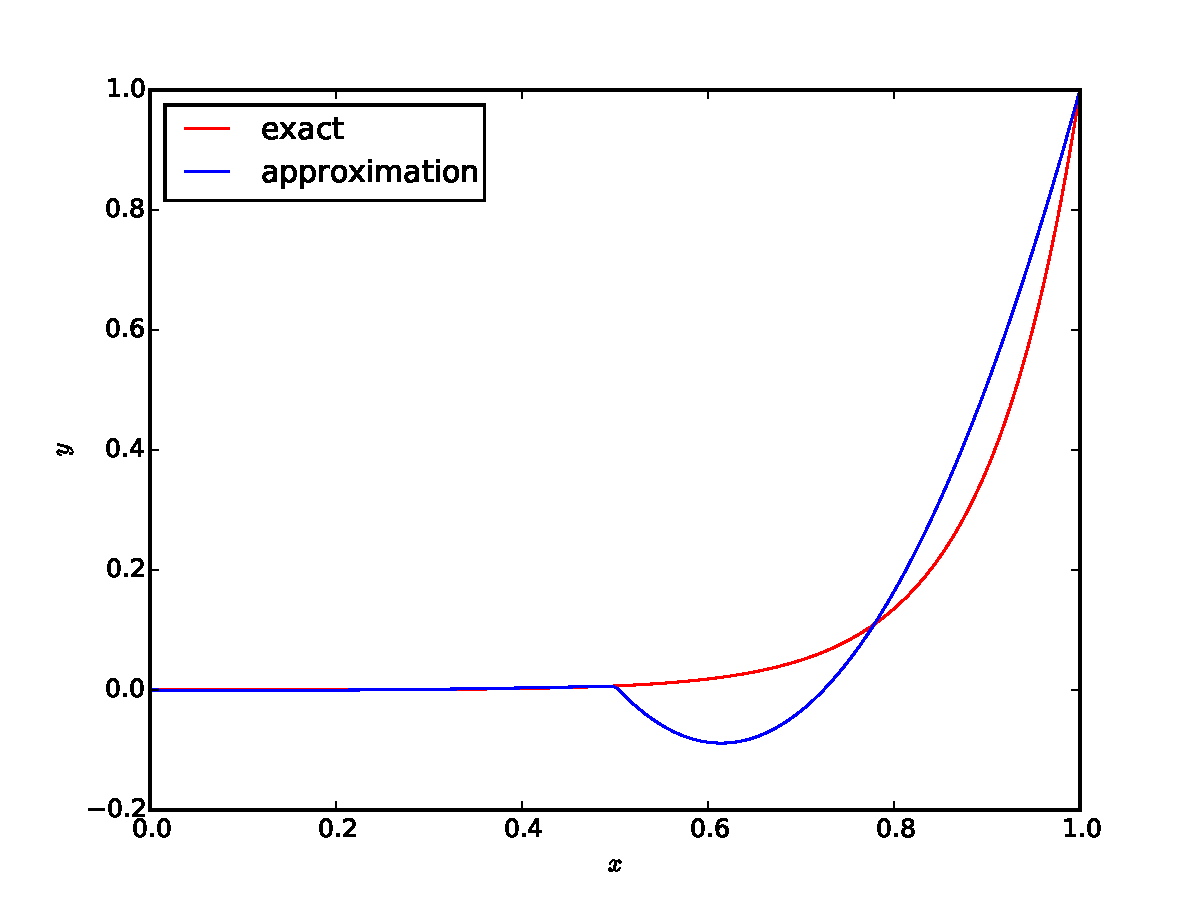
\includegraphics[trim = 0cm  0cm 0cm 0cm,clip,width=0.49\textwidth]{figures/optimalsolution_degree_2_Peclet_10}} 
	\caption{Optimal numerical solution in the $H^1_0$ semi-norm obtained using linear and quadratic continuous Petrov Galerkin with optimal testing on a partition of 2 elements.}
	\label{fig:optimaltestfunc3}
\end{figure}


\begin{figure}
	\centering
	\subfigure[$p = 1$]{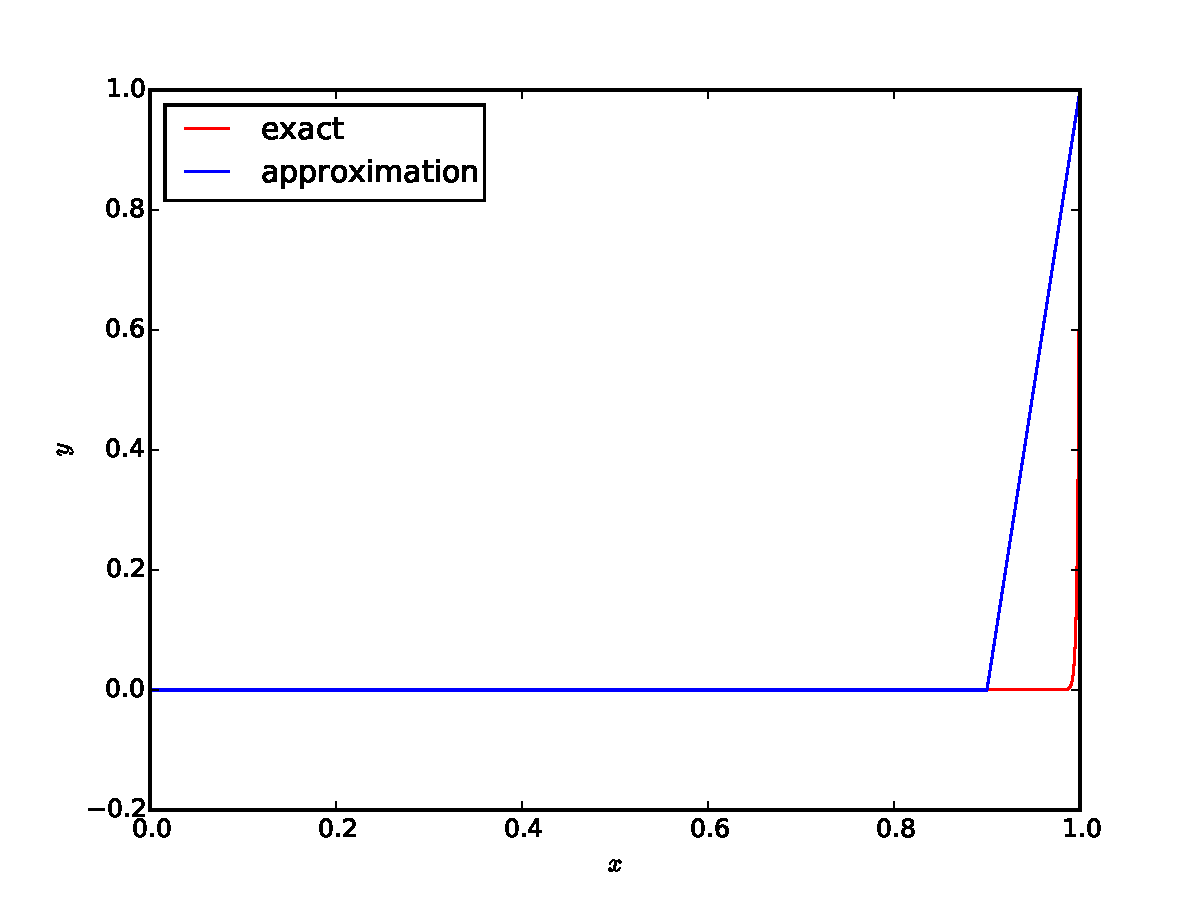
\includegraphics[trim = 0cm  0cm 0cm 0cm,clip,width=0.49\textwidth]{figures/optimalsolution_degree_1_Peclet_500_1}}
	\subfigure[$p = 2$]{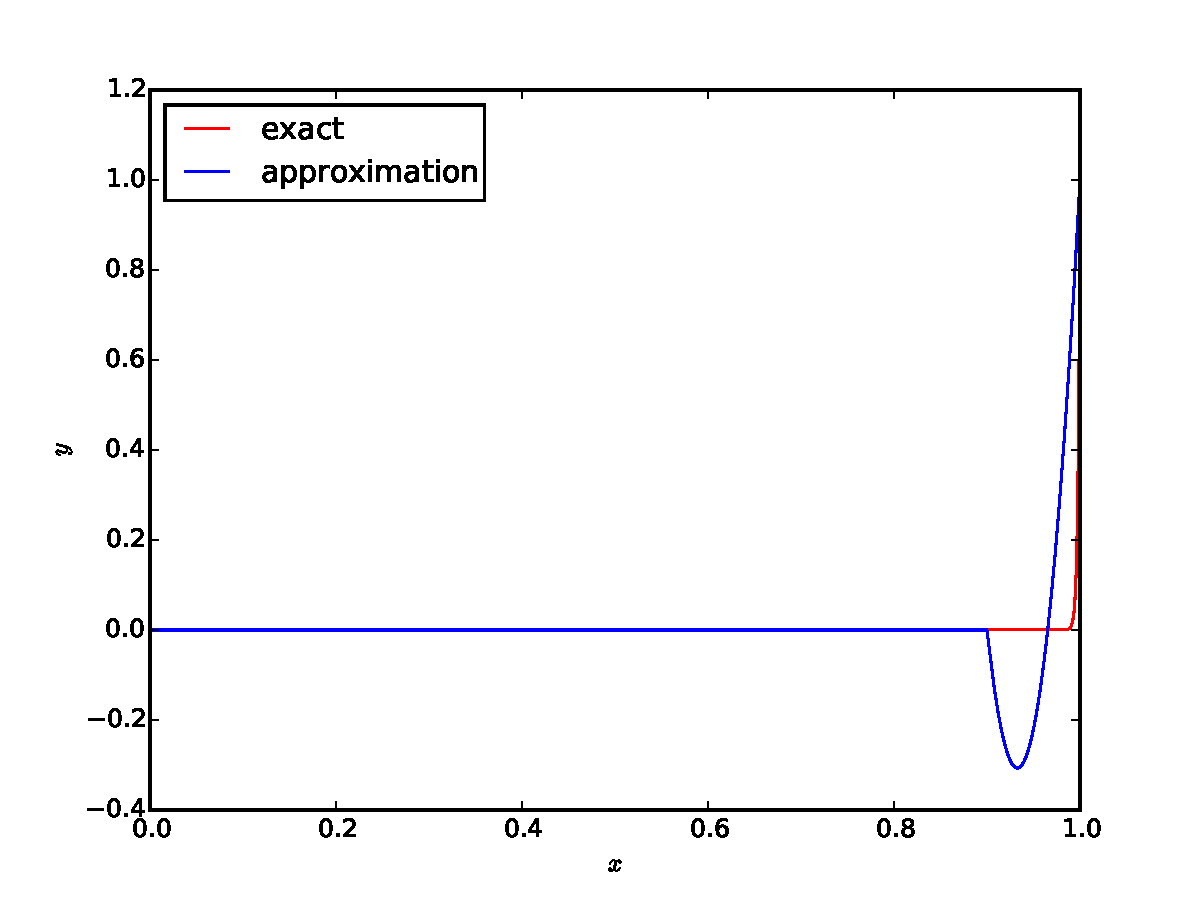
\includegraphics[trim = 0cm  0cm 0cm 0cm,clip,width=0.49\textwidth]{figures/optimalsolution_degree_2_Peclet_500_1}} 
	\caption{Test problem 1 with a zero right hand side and $Pe =500$. Optimal numerical solution in the $H^1_0$ semi-norm obtained using linear and quadratic continuous Petrov Galerkin with optimal testing  on a partition of 10 elements}
	\label{fig:optimaltestfunc4}
\end{figure}

\begin{figure}
	\centering
	\subfigure[$p = 1$]{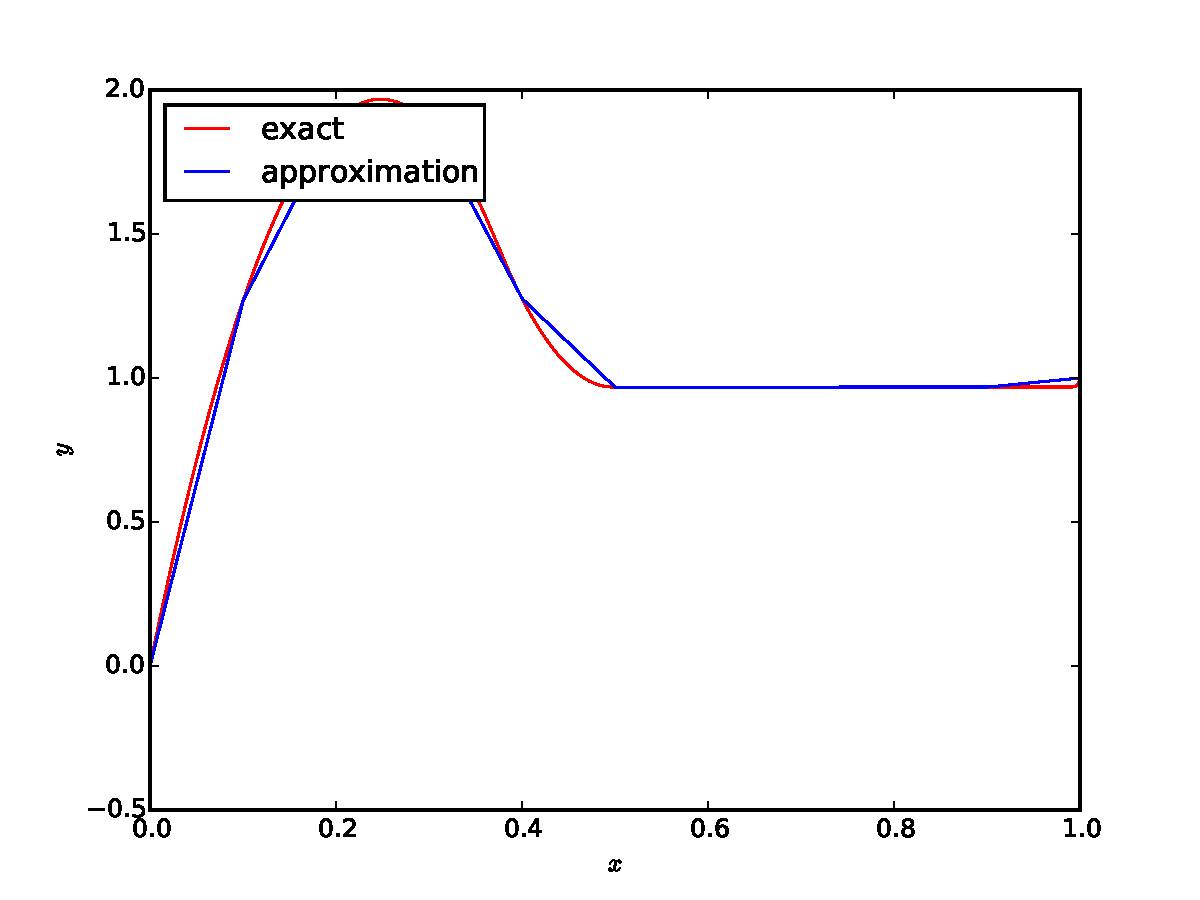
\includegraphics[trim = 0cm  0cm 0cm 0cm,clip,width=0.49\textwidth]{figures/optimalsolution_degree_1_Peclet_500_2}}
	\subfigure[$p = 2$]{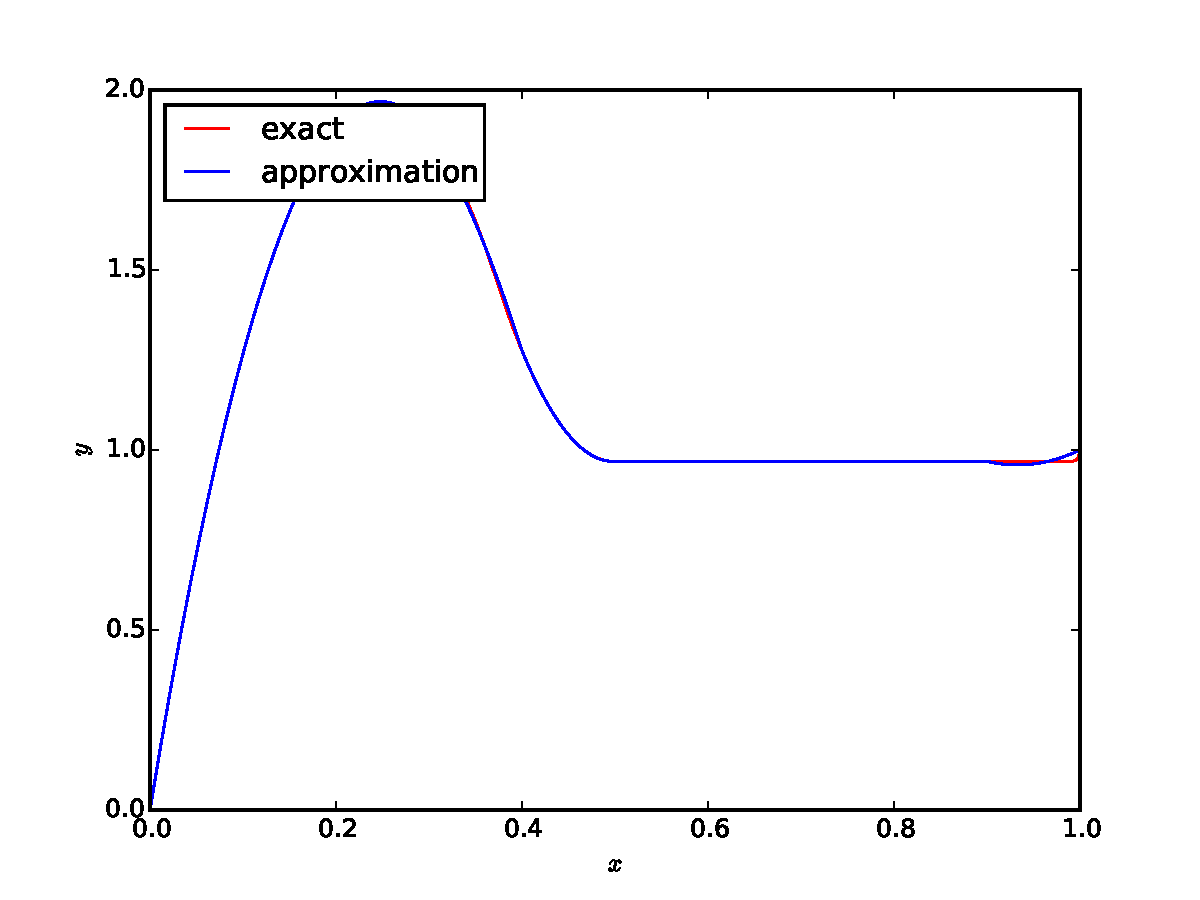
\includegraphics[trim = 0cm  0cm 0cm 0cm,clip,width=0.49\textwidth]{figures/optimalsolution_degree_2_Peclet_500_2}} 
	\caption{Test problem 2 with a non-zero right-hand-side and $Pe=500$. Optimal numerical solution in the $H^1_0$ semi-norm obtained using linear and quadratic continuous Petrov Galerkin with optimal testing  on a partition of 10 elements.}
	\label{fig:optimaltestfunc5}
\end{figure}

\subsection{A multi-scale perspective}
Using the scale decomposition in (\ref{eq:decomp}) we can decompose (\ref{eq:problem}) into the coarse and  fine scale equation, respectively,
\begin{align*}
	a(\bar{u} ,\bar{v}) + b(\bar{u},\bar{v})  + a(u',\bar{v}) + b(u',\bar{v}) &= l(\bar{v})  	& \forall \bar{v} \in \overline{V} \\
	a(\bar{u} ,v') + b(\bar{u},v')  + a(u',v') + b(u',v') &= l(v') 						& \forall v' \in V'
\end{align*}
Here we can observe that the fine scales are driven by the residual of the coarse scales. Ultimately we would like to somehow incorporate the effect of the fine scales in the coarse scale equation and obtain a good discrete approximation $\overline{u}$ with our coarse scale space. Typically, the fine scale equation is solved in an approximate way and its expression substituted into the coarse scale equation using static condensation.

We take an alternate approach and focus solely on the coarse scale equation. In terms of the basis functions $\phi_i, \; i = 1,2,...,n$ the coarse scale equation reads,
\begin{align*}
	a(\bar{u} ,\phi_i) + b(\bar{u},\phi_i)  + a(u', \phi_i) + b(u', \phi_i) = l(\phi_i) \quad \text{for } i = 1,2,...,n
\end{align*}
Comparing with the Petrov Galerkin method in (\ref{eq:problem2}),
\begin{align*}
	a(\bar{u} ,\phi_i) + a(\bar{u} ,\psi_i)  +  b(\bar{u},\phi_i) + b(\bar{u},\psi_i) = l(\phi_i) + l(\psi_i) \quad \text{for } i = 1,2,...,n
\end{align*}
We obtain the same result as in (\ref{eq:problem3}).


\subsection{Proposed direction}
Computation of optimal test functions is an expensive problem on its own: $n$ test functions need to be computed on a sub scale discretization local to the support of each function. For high Reynolds number flows this could become prohibitively expensive. Therefore we propose something remarkably similar to streamline upwind Petrov Galerkin (SUPG).

First note the following:
\begin{remark} Each function $\psi_i$ depends on,
	\begin{enumerate} 
		\item The trial function $\phi_i$.
		\item The local flow in $\mathrm{supp} \; \psi_i$, i.e. thing like,
		\begin{enumerate} 
			\item[(a)] Reynolds number
			\item[(b)] Direction of the velocity field with respect to the mesh.
			\item[(c)] The velocity gradient (expansion in one direction and contraction in the other)
			\item[(d)] Curvature of the flow.
		\end{enumerate}
	\end{enumerate}
\end{remark}
\begin{remark} In most finite element methods the trial functions are simply translated and scaled copies of one another.
\end{remark}

\begin{remark} The exact shape of the test functions is not important for stability. Only their action, i.e. $a(\cdot, \phi_i+\psi_i) + b(\cdot, \phi_i+\psi_i)$, matters. All functions in $V$ whose action is equal to that of the optimal test functions, $a(\cdot, \phi_i+\psi_i) + b(\cdot, \phi_i+\psi_i)$, form an equivalence class $V_{\overline{W}}$.
\end{remark}

What we propose is the following:
\begin{enumerate} 
	\item Construct a database of optimal test functions for a configuration space of flow fields, depending on Reynolds number, direction w.r.t. the mesh, etc.
	\item Compute their action, $a(\cdot, \phi_i+\psi_i) + b(\cdot, \phi_i+\psi_i)$, for each particular flow.
	\item Choose a particular candidate function (model) that is easy to evaluate and shares qualitative properties with the optimal test functions (e.g. the derivatives of the trial functions a la SUPG).
	\item Use regression or other machine learning techniques in order to tune the chosen candidate function (model) to obtain an element of $V_{\overline{W}}$.
\end{enumerate}

\begin{remark} Note the similarities with SUPG. In the one-dimensional setting of advection diffusion the velocity is a constant and depends solely on one parameter: the local Pecl\'et number. Optimal test functions are approximated by properly scaled derivatives of the gradient of the trial functions using a single parameter: the magical $\tau$. $\tau$ is tuned such that the new test functions are elements of the equivalence class $V_{\overline{W}}$.
\end{remark}

\begin{remark} In the multidimensional setting the local velocity field depends on more then just the Peclet number. Hence, we would require more then just a single tuning parameter in order to obtain elements of the equivalence class $V_{\overline{W}}$.
\end{remark}






